\section{Einleitung}
Die Entwicklung von \mops erfolgte in mehreren Schritten. Wichtige Zwischenstopps waren hier der Startprozess, die Interrupthandler, der Interrupt-Controller, die Interrupt-Service-Routinen und das Threadmanagment. Jeder dieser Punkte bedurfte einer einzelnen Entwurfsphase, auf die jetzt genauer eingegangen wird.
\section{Startmechanismus}
\label{e1:start}
Der Startprozess unterteilt sich in drei Schritte:

	\begin{figure}[h]
		\centering
					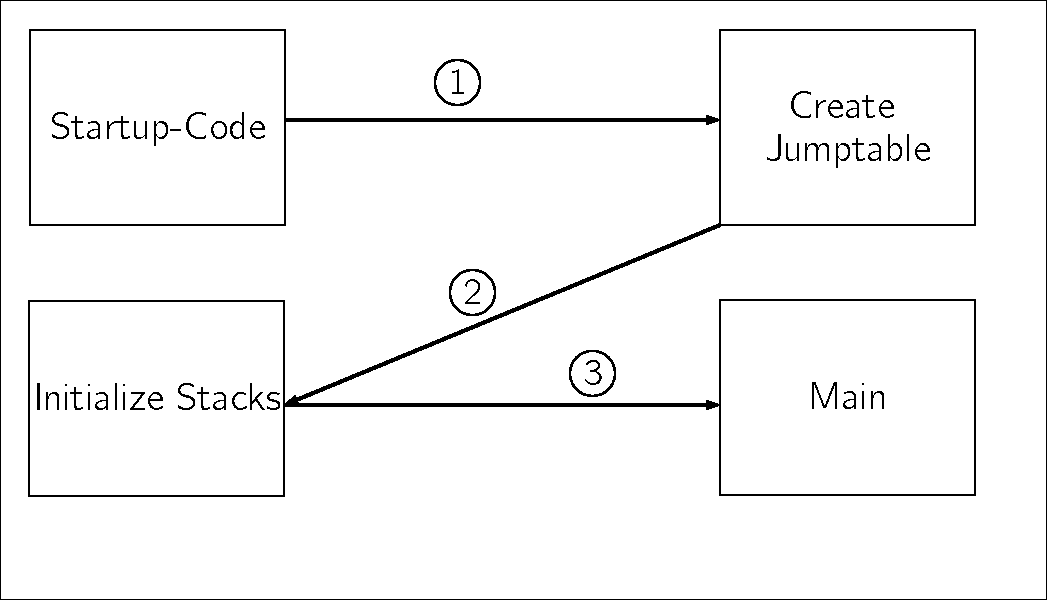
\includegraphics[scale=0.60]{common/kernel-img.pdf}	
		\caption{Kernel-Image Version 1}
		\label{draft:kernelImage}
	\end{figure}
	\begin{enumerate}
		\item{\textbf{Startup-Code}}\\
		 Der Emulator springt an die Adresse \texttt{0x000000}\footnote{\textit{Diese Adresse wird \"uber das Linker-Script bestimmt}}, an dieser Stelle steht die erste Assemblerroutine des Betriebssystems. Diese Routine dient dazu um gewisse Vorbedingungen zu erstellen. Eine davon ist die nachfolgende.
		 \item{\textbf{Interrupt Handler}}\\
		 \label{draft:exceptionHandler}
Interrupts k\"onnen von externen oder internen Ressourcen ausgel\"ost werden. Damit der Prozessor wei{\ss} wo er im Falle eines Interrupts hinspringen muss, schreibt ARM eine Struktur vor die eingehalten werden muss \parencite[vgl.][54]{archManI}. 
			\begin{figure}[h]
				\centering
					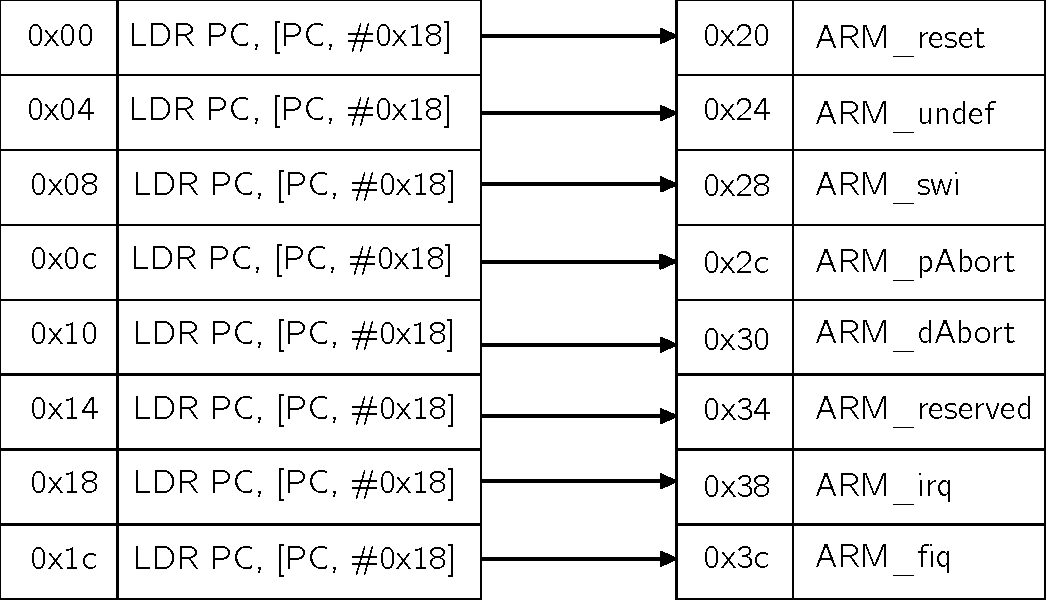
\includegraphics[scale=0.6]{common/exceptionhandler.pdf}
				\caption{Erzeugen der Sprungtabelle}
				\label{draft:excptionTable}
			\end{figure}\\
			In diesem Schritt ist erkennbar, dass es zwei Tabellen gibt die von dem Programmierer erstellt werden m\"ussen. Die erste Tabelle enth\"alt Programm-Relative Adressen auf eine zweite Tabelle. In der zweiten Tabelle befinden sich dann die konkreten Adressen der Interrupthandler. Neben des Interrupt f\"ur einen Reset des Systems gibt es noch weitere Interrupts wie die Undefined Operation (ARM\_undef), Softwareinterrupt (ARM\_swi), Prefetch-Abort (ARM\_pAbort), Data-Abort(ARM\_dAbort),  die Reserved Exception (ARM\_reserved) und ganz wichtig zu erw\"ahnen der IRQ (ARM\_irq und FIQ (ARM\_fiq).\\\\
Der Vorteil des Mechanismus, Programmrelative Adresse anstatt die direkten Handler zu laden, besteht darin das man so leicht die Handler austauschen oder zus\"atzliche hinzuf\"ugen kann ohne dabei den Assemblercode zu \"andern.\\
Neben der Erstellung der Sprungtabelle f\"ur die Interrupthandler, ist es weiterhin notwendig den Stack f\"ur die jeweiligen Prozessormodi zu definieren, dies geschieht im n\"achsten Schritt.
		\item{\textbf{Erstellung der Stacks mit anschlie\ss enden Sprung in main}}\\
		\label{draft:stack}
		Die f\"ur \mops relevanten Modi des Prozessors sind 
		\begin{dinglist}{227}
			\item{IRQ-Modus}
			\item{FIQ-Modus}
			\item{System-Modus}
			\item{Supervisor-Modus}
		\end{dinglist}
		Jeder dieser vier Modi, bis auf den System-Modus, hat seinen eigenen Stackpointer und f\"ur jeden muss dementsprechend der passende Stackpointer gesetzt werden. Das ist deshalb notwendig da im Falle einer Exception der Prozessor in den jeweiligen Modus wechselt und wenn kein valider Stackpointer vorhanden ist kann es zu undefinierten Verhalten kommen. Die Gr\"o\ss e der Stackpointer l\"asst sich \"uber das Link-File bestimmen, f\"ur \mops wurde eine Gr\"o\ss e von 8KB je Modus gew\"ahlt.\\
Sobald die Stacks alle initialisiert sind erfolgt der Sprung in die \texttt{main} Routine des Betriebssystem. Ab hier finden nun weitere Schritte statt um das System fertig zu initialisieren.
	\end{enumerate}
\section{Interrupt-Controller}
Ein Interrupt-Controller stellt in einem Betriebssystem die Schnittstelle zwischen den Interrupts und der Hardware dar Er priorisiert die Interrupts, die von externen wie auch internen Quellen ausgel\"ost werden k\"onnen, und leitet sie an das Betriebssystem weiter. Es gibt zwei Arten von Controllern:
\begin{dinglist}{227}
	\item{Non-Vectored Interrupt-Controller}
	\item{Vectored Interrupt-Controller}
\end{dinglist}
Die erste Version, \textbf{Non-Vectored Interrupt-Controller}, stellt nur die M\"oglichkeit bereit einen Interrupt abzufangen, jedoch muss sich der Programmierer darum k\"ummern welche Quelle den Interrupt ausgel\"ost hat, die Priorit\"at ermitteln und die passende Interrupt-Service Routine herausfinden. Das klingt zwar im ersten Moment ganz logisch und sinnvoll, ist aber mit einer Menge Code verbunden und stellt deshalb eine sehr gro\ss e Fehlerquelle dar.\\
Der Vectored Interrupt-Controller ist eine, in Hardware gegossene, Komponente auf dem Board welches man direkt benutzen kann. Er bietet die Konfigurationsm\"oglichkeit, zu definieren welche Interrupts von welchen Quellen ausgel\"ost werden k\"onnen, welche Priorit\"aten sie haben und welche Interrupt-Service Routinen f\"ur diese Interrupts zur Verf\"ugung gestellt werden. Nun brauch man im Falle eines Interrupts keine umfangreichen Mechanismen lostreten um die Quellen zu ermitteln, sondern der Interrupt-Controller stellt jetzt alle diese Informationen bereit. Die Installations dieses Controllers ist zwar komplexer als die der ersten Version, aber die M\"oglichkeiten sind breiter und die Benutzung ist komfortabler. Aus diesen Gr\"unden wurde sich bei \mops f\"ur den \textbf{Vectored Interrupt Controller} entschieden.
Das folgende Bild ist eine schematische Darstellung des Vectored Interrupt-Controller.

\begin{figure}[H]
	\begin{center}	
	\caption{Vectored Interrupt Controller - relevante Register}
	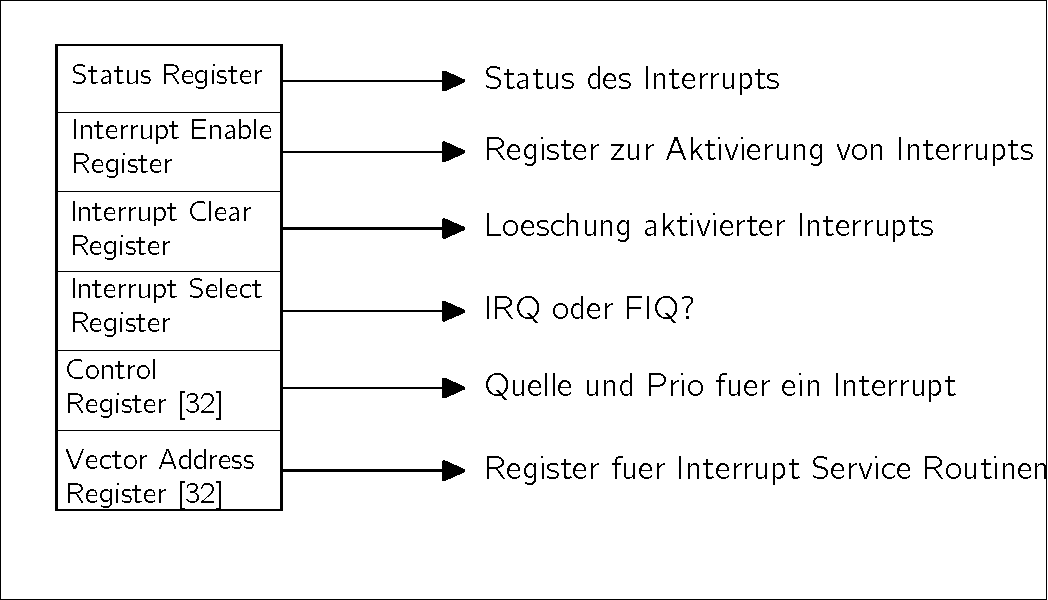
\includegraphics[scale=0.60]{common/vic.pdf}
	\end{center}
	\label{vicSchema}
\end{figure}
\noindent
Sofern das Board einen Vectored Interrupt-Controller zur Verf\"ugung stellt ist dieser an einer bestimmten Adresse lokalisiert. Bei dem von \mops emulierten System ist dies die Adresse \texttt{0x10140000}\parencite[vgl.][223]{archManI}. Ab dieser Adresse beginnt der Adressbereich des Controllers, hier befinden sich oben genannte Register wie Statusregister, Interrupt Enable Register, Interrupt Clear Register, Interrupt Select Register etc., desweiteren sind hier auch die f\"ur die Interrupt Vectoren wie auch die Control Register f\"ur die jeweiligen Interrupts \parencite[vgl.][35]{vic}.\\\\
Die relevanten Register f\"ur \mops sind die Vector Address Register, Control Register, Interrupt Enable, Interrupt Clear und Interrupt Select Register. \"Uber diese ist es m\"oglich die Service Routinen f\"ur die Interrupts zu definieren, wie auch die Priorit\"aten und ob der konfigurierte Interrupt als ein IRQ oder FIQ behandelt werden soll. Mit der folgenden Grafik wird schematisch dargestellt wie eine Konfiguration des Controllers aussehen kann.
\begin{figure}[H]
	\begin{center}	
	\caption{Konfiguration am Beispiel eines Timer Interrupt}
	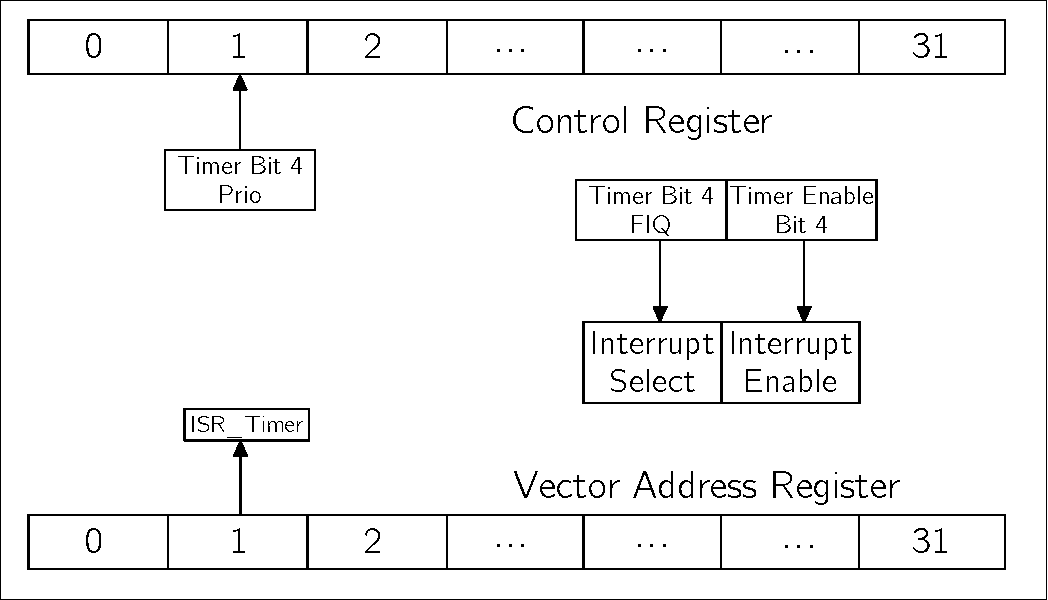
\includegraphics[scale=0.60]{common/vicsample.pdf}
	\end{center}
	\label{draft:vicSample}
\end{figure}
\newpage
\noindent
Dieses Beispiel zeigt eine Beispielkonfiguration des Timerinterrupts. Um diesen Interrupt zu konfigurieren sind vier Schritte notwendig:
\begin{dinglist}{227}
	\item{Aktivierung des Interrupts im \textit{Interrupt Enable Register}. F\"ur den Timer-Interrupt muss hier das 4. Bit gesetzt werden \parencite[vgl.  Tabelle 4-40][227]{archManI}}
	\item{Das \textit{Interrupt Select Register} muss auf 1 gesetzt werden um den Timer Interrupt als FIQ zu konfigurieren \parencite[vgl Tabelle 3-5][39]{vic}.}
	\item{In dem \textit{Control Register} muss an der Array Stelle 1 das 4. Bit gesetzt werden um die Quelle von dem Timer-Interrupt zu definieren.}
	\item{In dem \textit{Vector Address Register} muss an der Array Stelle 1 die Adresse der Interrupt Service Routine f\"ur den Timer-Interrupt eingetragen werden.}
\end{dinglist}


\section{Interrupt-Service Routinen}
Nachdem die Interrupts konfiguriert wurden ist es notwendig die Interrupt-Service Routinen der Interrupts zu definieren. Beispielhaft werden hier die Routinen des Timers und des UART0-Interrupts pr\"asentiert.
\begin{figure}[H]
	\begin{center}	
	\caption{Interrupt Service-Routinen Timer \& UART0}
	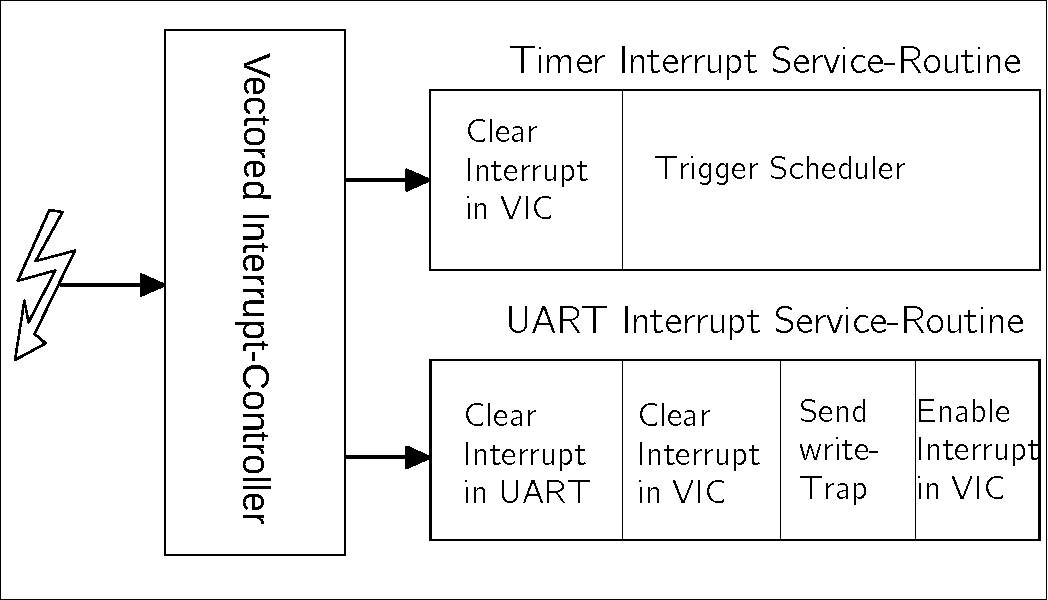
\includegraphics[scale=0.60]{common/isr.pdf}
	\end{center}
\end{figure}
\noindent
Sobald der Interrupt ausgel\"ost wurde behandelt der Controller diesen und leitet es an die zugeh\"orige Routine zur Behandlung weiter. Im Beispiel des Timers, wird hier der Interrupt erst im Controller auf 'Behandelt' gesetzt und dann wird der Scheduler aufgerufen um dem n\"achsten Prozess zu starten. Das L\"oschen des Interrupts im Controller ist deshalb erforderlich, damit ein neuer Interrupt ausgel\"ost werden kann, denn nur nachdem der Interrupt als behandelt markiert wurde, kann ein neuer erzeugt werden. \\ In der aktuellem Implementation von \mops gibt es zwei Interrupts auf die reagiert wird. Zum einen ist das der \textit{Timer0}-Interrupt und zum anderen der Interrupt des \textit{UART0}-Interface. Bei Bedarf kann man auch noch weiter Interrupts definieren, dazu muss jedoch die Konfiguration des VIC abg\"andert werden.
\section{Syscalls}
Neben den IRQ und FIQ spielen die Syscall auch noch eine sehr wichtige Rolle. Um einen Syscall aufzurufen ist es notwendig eine sogenannte SWI - \textit{Software Interrupt} Instruktion auszuf\"uhren. Diese Instruktion wird von einem Handler aufgefangen und dort wird entschieden welcher Syscall ausgef\"uhrt wird.\\
Ein SWI ist eine Instruktion die nicht im Kernel-Modus l\"auft aber Kernel-Routinen aufrufen darf. Das ist dann sinnvoll, wenn ein User-Programm Zugriff auf eine Kernel-Routine (wie das Schreiben auf die Konsole) ben\"otigt. Wie in Abbildung \ref{draft:excptionTable} zu erkennen ist, wird bei einer SWI-Instruktion die ARM\_swi Routine angsprungen. Diese Routine leitet den Request an eine weitere Komponente weiter die schematisch wie folgt aussieht.
\begin{figure}[H]
	\begin{center}	
	\caption{SWI-Handler}
	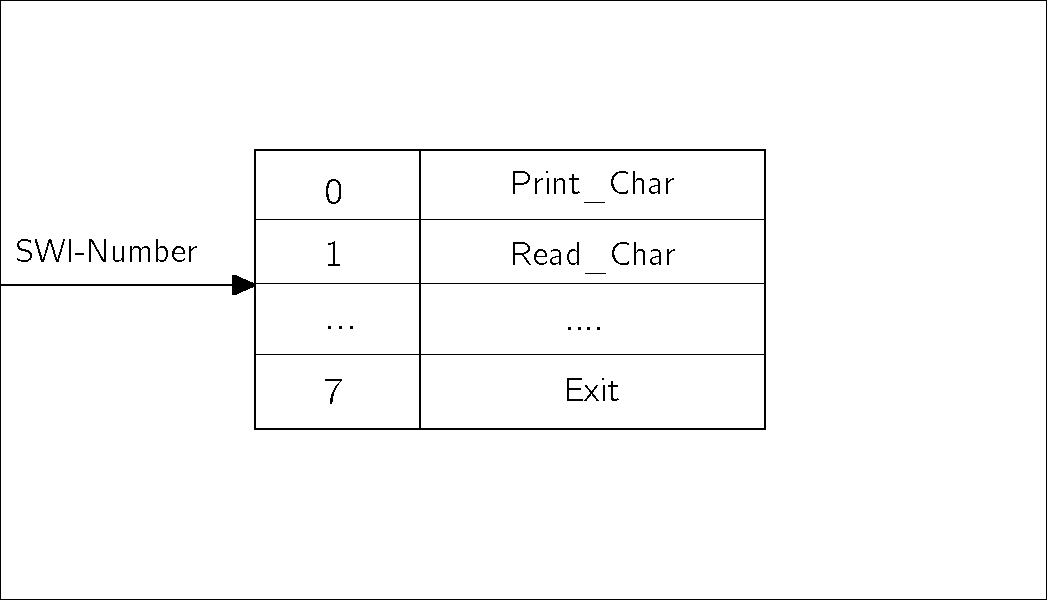
\includegraphics[scale=0.60]{common/swihandler.pdf}
	\end{center}
\end{figure}
\noindent
In der aktuellen Fassung von \mops ist nur der SWI-Handler f\"ur den \texttt{Print\_Char}-SWI definiert, es sollen jedoch weitere folgen. Ein Syscall hat immer ein gewisse Anzahl von Parameter, da f\"ur \mops nur \texttt{Print\_Char} implementiert wurde reicht es hier nur die Parameter von dieser Methode zu beschreiben.\\ 
Der Parameter f\"ur den beschrieben Syscall besteht im Groben und Ganzen nur aus einem Parameter, der Character der auf der Console ausgegeben werden soll.
\newpage
\section{Threadmanagment}
Das Threadmanagment stellt die Verwaltung der Threads in einem System dar. Das bedeutet wie wechseln sich die Threads ab und von was k\"onnen sie unterbrochen werden . Wie diese Prozesse miteiander arbeiten, soll in der folgenden Grafik verdeutlicht werden.
\begin{figure}[H]
	\begin{center}	
	\caption{\"Ubersicht Threadmanagement}
	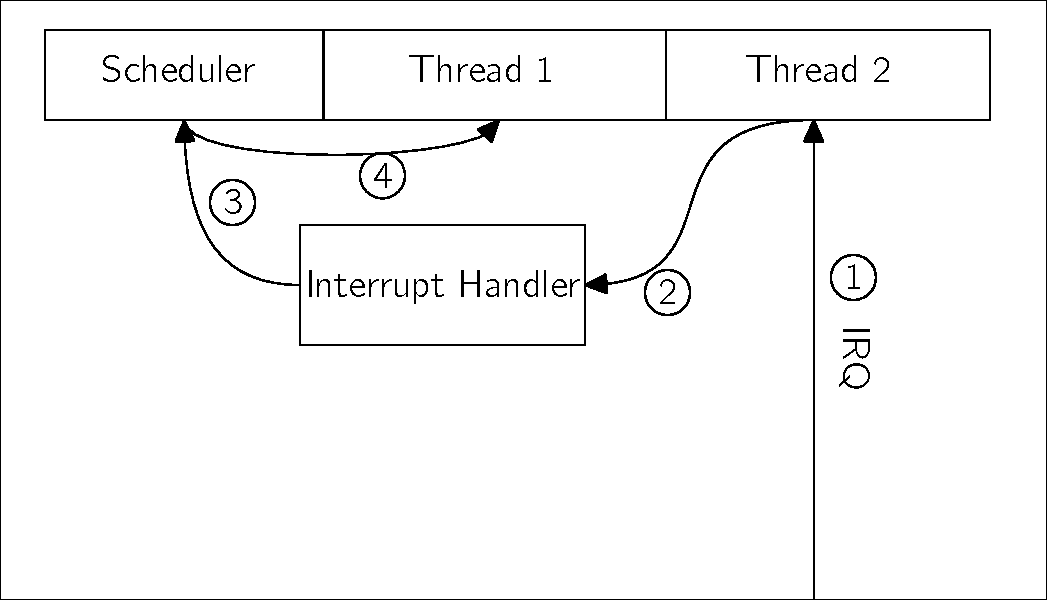
\includegraphics[scale=0.60]{common/draftconcrete-thread-managment.pdf}
	\end{center}
\end{figure}\noindent
Die Ausgangsituation ist ein System in dem drei Threads koexistieren k\"onnen. Jeder dieser Threads hat, aufgrund des Scheduling-Verfahren, nur eine gewisse Zeit in der er arbeiten darf. Nun kommt ein Interrupt rein und unterbricht den aktuellen Thread, hier mit 1 beschrieben. \\
Der Thread wird unterbrochen und es wird der Interrupthandler f\"ur diesen Interrupt aufgerufen, z.B. der Timer-Interrupthandler. Bei Punkt zwei ist dieser Interrupt-Handler dargestellt. Er ruft im dritten Schritt den Scheduler auf. Der Scheduler ermittelt dann, basierend auf dem Scheduling-Verfahren, den n\"achsten Thread der die Kontrolle bekommt, was hier im 4. Schritt stattfindet. 
\subsection{Threadlayout}
Das Threadmanagment spielt eine wichtige Rolle in jedem Betriebssystem. Aufgrund der Komplexit\"at und des zeitlichen Faktors wurde bei \mops auf ein rudiment\"areres System gesetzt. Das bedeutet das keine Threads zur Laufzeit des Systems geladen werden k\"onnen sondern die Threads vor Beginn definiert werden mussten.\\
Eine abstrakte Darstellung dieses Thread-Image kann man sich wie folgt vorstellen:
\begin{figure}[H]
	\begin{center}	
	\caption{Thread-Image}
	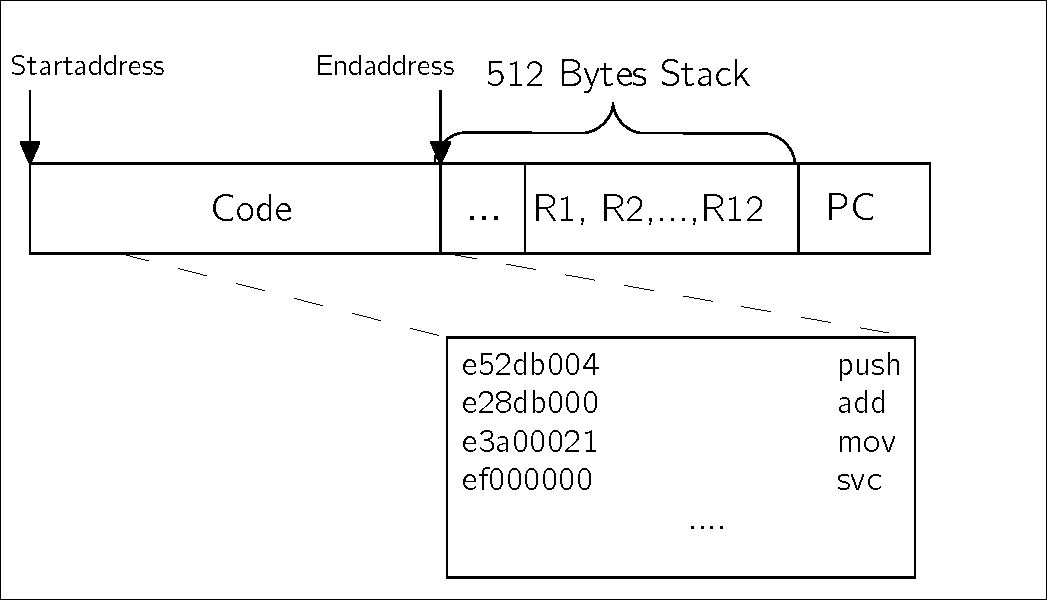
\includegraphics[scale=0.60]{common/threadimage.pdf}
	\end{center}
\end{figure}
\noindent
Diese Struktur wird zu Begin des Betriebssystem im RAM hergestellt. Zuvor muss jedoch doch der Assemblercode aus dem zu ladenen Thread extrahiert werden. Die Threads werden als einfache C-Programme dargestellt. Diese C-Programme werden so rudiment\"ar wir m\"oglich Kompiliert und gelinkt, das bedeutet das s\"amtliche Standardbibliotheken nicht mit gelinkt werden und keine main-Funktion bereitgestellt wird. Die entstandene .ELF-Datei wird dann ins Bin\"arformat umkopiert und danach extrahiert ein Programm den Assemblercode aus der Bin\"ardatei und schreibt diese in eine RAM-Disk. F\"ur \mops wurde eine sehr proprit\"are RAM-Disk gew\"ahlt. Folgende Grafik zeigt eine schematische Darstellung dieser RAM-Disk. 
\begin{figure}[H]
	\begin{center}	
	\caption{RAM-Disk}
	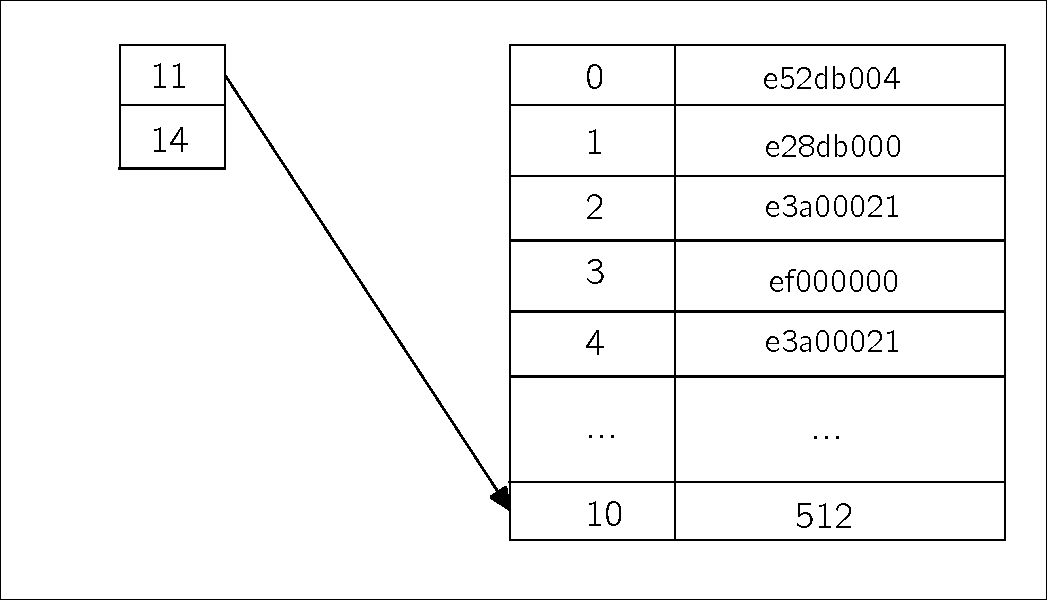
\includegraphics[scale=0.60]{common/ramdisk.pdf}
	\label{ramdisk}
	\end{center}
\end{figure}
\noindent
Nachdem diese RAM-Disk erstellt wurde, kann \mops diese im Betrieb laden und den Assemblercode an die passende Position im RAM laden. Neben den Informationen \"uber den Assembler-Code enth\"alt die RAM-Disk unter anderem die Information wieviel Bytes an Stack f\"ur den Prozess reserviert werden. Dieser Bereich wird dann beim kopieren vorerst nur mit Nullen aufgef\"ullt. \\
Um die M\"oglichkeit offen zu halten mehr als einen Prozess in den RAM zu laden, stellt die RAM-Disk eine weitere Tabelle zur Verf\"ugung in welcher die Informationen zur L\"ange jeder einzelnen Threads eingetragen sind. F\"ur Abbildung \ref{ramdisk} bedeutet dass, das der erste Thread eine L\"ange von 11 aufweist und ab dem 12. Eintrag der n\"achste Thread beginnt.
\subsection{Scheduling}
Sobald der Thread in den RAM geladen wurde, kann das Betriebssytem jetzt den ersten dieser Prozesse starten. Dieser Start manifestiert sich dadurch das der Stackpointer, vom Kernel auf den Start-Bereich des neuen Stacks von dem Thread, umgemappt werden muss. Danach werden alle Register auf dem neuen Stack gesichert und es erfolgt ein Sprung in die Routine die zuletzt aus der RAM-Disk geladen wurde. 
\begin{figure}[H]
	\begin{center}	
	\caption{RAM-Disk}
	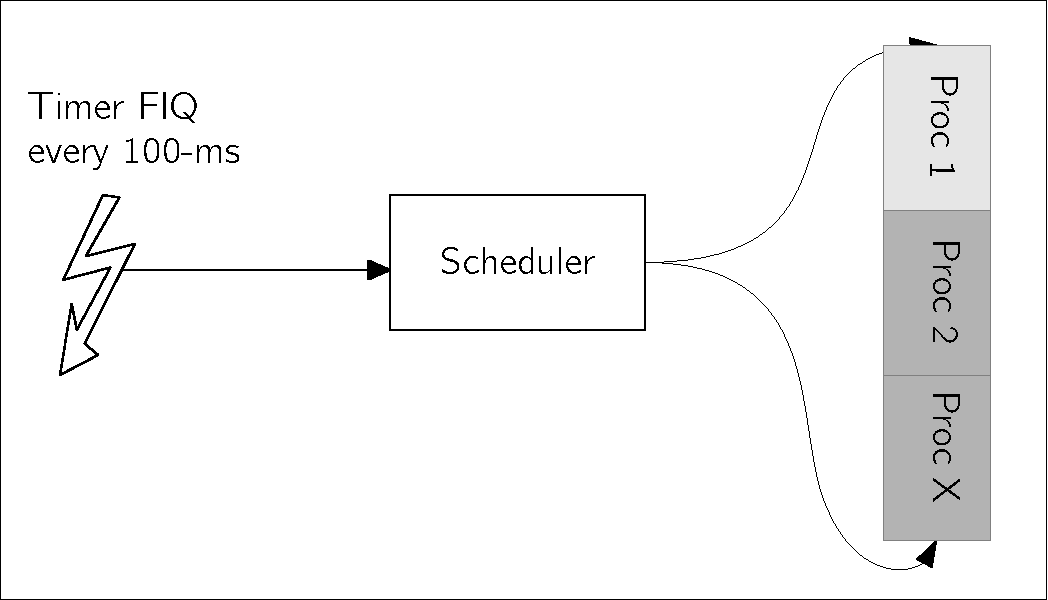
\includegraphics[scale=0.60]{common/scheduler.pdf}
	\label{scheduler}
	\end{center}
\end{figure}
\noindent
In Grafik \ref{scheduler} wird veranschaulicht wie der Mechanismus, des Thread-Umschalten, in \mops umgesetzt wurde. Hier sieht man das aller 100ms der Timer-Interrupt ausgel\"ost wird und dieser startet den Scheduler. Der Scheduler sucht dann den n\"achsten wartenden Prozess, hier Gelb, raus und schaltet diesen ein. Der andere, momentan gr\"une, wird dann in den wartenden Status geschalten.
Es gibt einige bekannte Scheduling-Verfahren in modernen Betriebssystemen, viele dieser Verfahren kooperieren auch unter bestimmten Umst\"anden um die beste Performance herauszuholen. Hier sind ein paar der wichtigsten Verfahren etwas n\"aher beschrieben:
\begin{dinglist}{227}
	\item{\textbf{First-Come First-Serve}} \\
	Dieses System kann man sich wie eine Schlange an der Post vorstellen. Prozesse werden in eine Queue\footnote{Eine weitverbreitete Datenstruktur in modernen Programmiersprachen die nach dem \textit{First-In First-Out} Prinzip funktioniert.} gepackt und von dort bearbeitet. Dieses System hat jedoch den Nachteil das lange Wartezeiten, durch Prozesse die die CPU sehr \"uberdurschnittlich lange in Anspruch nehmen, entstehen k\"onnen.\newpage
	\item{\textbf{Shortest-Job-First}}\\
	W\"ahrend bei diesem Verfahren darauf abgezielt wird den Prozessen die CPU-Zeit zu \"uberlassen welche am k\"urzesten sind. Wie in \cite[189]{scheduling} geschrieben 
\begin{quote}
	\textquote{\textit{This  algorithm associates with each process  the length of the 
process's next CPU burst.}}
\end{quote}
versucht dieser Algorhithmus anhand der CPU-Bursts\parencite[vgl.][184]{scheduling} zu ermitteln wie lange ein Prozess in etwa ben\"otigen wird. Anhand dieser Informationen wird also dann der n\"achste Prozess ermittelt der an der Reihe ist.
Sollten jedoch zwei Prozesse die gleichen CPU-Bursts haben, so wird das \textit{First-Come First-Serve} Verfahren angewendet. Der Vorteil hier ist nat\"urlich das es wesentlich optimaler als die vorherig genannten, jedoch ist es auch komplizierter zu implementieren.
\item{\textbf{High-Priority First}}\\
Mit diesem Verfahren ist es m\"oglich Threads mit Priort\"aten zu versehen und anhand dieser Priorit\"aten kann der Scheduler dann den n\"achsten Thread ermitteln der die CPU-Zeit bekommt. Aber auch hier gibt es einen Nachteil. Was ist wenn alle Threads eine hohe Priorit\"at haben? Das bedeutet das dieses Verfahren nur in Kombination mit einem anderen Verfahren umsetzbar ist, denn es muss noch eine weitere Eigenschaft geben anhand der ein Thread ausgew\"ahlt werden muss, da sonst Probleme entstehen.
	\item{\textbf{Round-Robin}}\\
	Dieses Verfahren 
		\textquote{\textit{is designed especially for  time-
sharing systems.}}\parencite[vgl.][194]{scheduling}
Das bedeutet das der Algorhitmus eine kleine Zeitscheibe definiert in der der Prozess die CPU bekommt. Danach werden die Prozesse die sich in der ``Ready-Queue'' befinden abgearbeitet und jeder bekommt f\"ur die vorher bestimmte Zeit die CPU. Diese Queue wird als eine Ring-Liste behandelt, das hat den Effekt das der Scheduler immer wieder jeden Prozess kurz rannimmt. Der Vorteil dieses Mechanismus ist das jeder Prozess gleich bewertet wird und das es relativ einfach zu implementieren ist. Jedoch bringt genau dieser Vorteil auch einen Nachteil mit sich, n\"amlich das Prozesse die eigentlich eine l\"angere Zeitschreibe br\"auchten immer warten m\"ussen bis sie wieder am Zug sind und das kann nat\"urlich zu sehr hohen Latenzen in der Ausf\"uhrung kommen.
\end{dinglist}
Es wurden jetzt eine Reihe von Scheduling-Mechanismen vorgestellt und es musste eine Entscheidung f\"ur \mops getroffen werden. Aufgrund der einfachen Implementation, fiel die Wahl auf das \textbf{Round-Robin} Verfahren. Die Nachteile konnten f\"ur die erste Version von \mops vernachl\"assigt werden.
